\chapter{Implementation of Extended Kalman Filter}
\label{chap:ekf}
\section{Theory of Kalman Filters \& EKF}

The motivation of Rudolf Kalman for deriving the Kalman filters was to improve the accuracy of estimation and prediction of states using a probabilistic filter. The Kalman filter works on the principle of predicting the current states of a system based on either a static or dynamic mathematical state space model of the plant and the previously estimated state and then perform correction using current measured states. The accuracy of the filter therein lies in the appropriate physcial plant modelling and fine tuning of the relevant covariance matrices of measurement and process noise.

\subsection{State Space Systems}
The state space refers to the mathematical model of a physical system described using a set of variables which are related by first order differential or difference equation. The variables involved are known as \textbf{state variables} and the system state defined by them is called \textbf{state} in short.

\subsection{Random Noise and Probability Distributions}

Every physical phenomenon in nature can be measured using modern sensors and mechanical devices. The measurement of any state/path variable embeds a certian noise of uncertainty in the measurement campaign. This is mostly due to the accuracy of sensors. this noise is accompanied by yet another uncertainity of unmodelled disturbances, as the state of a dynamic system constantly changes with time. The mathematical approach for handling uncertainties is highlighted by probabilistic distributions. The probability curve for an ideal measurement campaign with infinite instances of data measurement tends towards a normal distribution as dictated by Central Limit Theorem. The normal distribution of any quantity is described using the mean and the standard deviation.

The linear Kalman Filter models the measurement noise and the process noise seperately and evaluated them using a factor known as Kalman Gain. this factor could show the balance or trusting tendency between measurement data point and the prediction data point. The factor is updated after every iteration of calculation and is used to update the filter matrices.

The disadvantage of Linear Kalman Filter lies in handling the state space plant models with non-linear differential equations, In EKF however the linearisation is performed dynamically around the current state estimate for every time step using first order taylor series expansion(the Jacobian matrices). This also signifies that the probability distribution of non-linear plants is also non-Gaussian and cannot be depicted using normal distribution. 

\subsection{One-Dimensional Linear Kalman Filter}
\label{sec:kalman_filter_1d}

In one-dimensional state estimation, the Kalman filter operates as a cyclic two-phase algorithm consisting of a \enquote{Predict} phase (extrapolation) and a \enquote{Correct} phase (update).~\cite{CC17}%
\sidenote{$\hat{x}_{n,n}$ denotes the current state estimate at discrete time step $n$ after taking measurement $z_n$, while $\hat{x}_{n+1,n}$ represents the predicted state for the next time step but derived at current time step. Similarly, $p_{n,n}$ is the estimate variance (uncertainty), $r_n$ is the measurement variance, and $q_n$ is the process noise variance.}

The filter is statistically optimal because it combines prior predictions and noisy sensor measurements in a manner that provably minimizes the estimation uncertainty $p_{n,n}$. The filter also requires Initial values of $\hat{x}_{0,0}$ and its variance $p_{0,0}$, Choosing an excessively high initial variance (e.g., $p_{0,0}=10{,}000$) will lead to longer convergence times, whereas setting it too low can cause estimator overconfidence

The following five equations define the complete recursive loop for a linear system:

\begin{enumerate}[label=\textbf{Step \arabic*:}, leftmargin=*, itemsep=1em]
	
	\item \textbf{State Extrapolation (\emph{Predict})}\\
	This step extrapolates the current system state estimate forward to the next time step/iteration cycle using the governing dynamic model of the plant. For constant velocity dynamics, the position advances by the estimated velocity multiplied by the time interval $\Delta t$, while velocity remains constant.
	\begin{equation}
		\begin{split}
			&\hat{x}_{n+1,n} = \hat{x}_{n,n} + \Delta t \hat{\dot{x}}_{n,n} \\ 
			& (\text{or } \hat{x}_{n+1,n} = \hat{x}_{n,n} \text{ for constant dynamics})
		\end{split}
	\end{equation}
	
	\item \textbf{Covariance Extrapolation (\emph{Predict})}\\
	This step extrapolates the estimate variance ahead in time to account for uncertainty introduced during the transition interval.%
	\sidenote{Alternative literature designations for process noise variance $q_n$ include plant noise, driving noise, dynamics noise, model noise, and system noise.}\\
	Combines the baseline uncertainty of the current estimate with the additive process noise variance ($q_n$).
	\begin{equation}
		\begin{split}
			&p_{n+1,n} = p_{n,n} + q_n \\ 
			& (\text{or } p_{n+1,n}^x = p_{n,n}^x + \Delta t^2 p_{n,n}^v + q_n \text{ for constant velocity})
		\end{split}
	\end{equation}
	
	\item \textbf{Kalman Gain (\emph{Update})}\\
	Then compute the optimal weighting coefficient between zero and one that balances trust between the prior prediction and the new sensor data.\\
	 It evaluates the ratio of the prior extrapolated estimate variance against the total system uncertainty, including measurement variance ($r_n$).
	\begin{equation}
		K_n = \frac{p_{n,n-1}}{p_{n,n-1} + r_n}
	\end{equation}
	
	\item \textbf{State Update (\emph{Update})}\\
	Now refine the prior state estimate by incorporating the actual sensor measurement ($z_n$) sampled at the current cycle.\\
	Adjusts the prior prediction by the measurement residual (innovation), scaled precisely by the calculated Kalman Gain.
	\begin{equation}
		\hat{x}_{n,n} = \hat{x}_{n,n-1} + K_n\left(z_n - \hat{x}_{n,n-1}\right)
	\end{equation}
	
	\item \textbf{Covariance Update (\emph{Update})}\\
	Finally update the estimate variance of the current state to reflect the reduction in uncertainty after consuming the measurement.%
	\sidenote{Because $(1 - K_n) \le 1$, the estimate variance $p_{n,n}$ strictly decreases during each update, driving the filter toward steady-state convergence.}\\
	Scales the prior extrapolated variance down by the complementary factor $(1 - K_n)$ to ensure estimator convergence over time.
	\begin{equation}
		p_{n,n} = (1 - K_n)p_{n,n-1}
	\end{equation}
	
\end{enumerate}


\paragraph{Extension to Non-Linear Systems: The Extended Kalman Filter}
\label{sec:extended_kalman_filter}

When the underlying system dynamics or sensor relationships are non-linear, the simple scalar arithmetic is generalized into the Extended Kalman Filter (\textsc{Ekf}).%
\sidenote{To propagate estimate uncertainties through non-linearities without distortion, the \textsc{EKF} applies a first-order Taylor series expansion around the current estimate, generating partial derivative slope terms (Jacobians).}
the linear steps are replaced by introducing non-linear state and measurement functions, $f(\cdot)$ and $h(\cdot)$, alongside their respective \textbf{Jacobian derivatives, $F_n$ and $H_n$.}


\begin{enumerate}[label=\textbf{Step \arabic*:}, leftmargin=*, itemsep=1em]
	
	\item \textbf{Non-Linear State Extrapolation (\emph{Predict})}\\
	Extrapolates the state estimate directly through the non-linear dynamic model function $f(\cdot)$ using known control inputs $u_n$.
	\begin{equation}
		\hat{x}_{n+1,n} = f\left(\hat{x}_{n,n}, u_n\right)
	\end{equation}
	
	\item \textbf{Linearized Covariance Extrapolation (\emph{Predict})}\\
	Propagates the estimate variance using the dynamic model Jacobian slope $F_n$, evaluated at the current state estimate, plus process noise variance $q_n$.
	\begin{equation}
		p_{n+1,n} = F_n p_{n,n} F_n^\top + q_n \; \text{where} \; F_n = \left. \frac{\partial f}{\partial x} \right|_{\hat{x}_{n,n}, u_n}
	\end{equation}
	
	\item \textbf{Kalman Gain (\emph{Update})}\\
	Computes the optimal weighting coefficient by substituting the linearized measurement Jacobian slope $H_n$ into the variance ratio.
	\begin{equation}
		K_n = p_{n,n-1} H_n^\top \left(H_n p_{n,n-1} H_n^\top + r_n\right)^{-1} \quad \text{where} \quad H_n = \left. \frac{\partial h}{\partial x} \right|_{\hat{x}_{n,n-1}}
	\end{equation}
	
	\item \textbf{Non-Linear State Update (\emph{Update})}\\
	Refines the prior prediction by evaluating the measurement residual (innovation) directly against the non-linear measurement function $h(\cdot)$.
	\begin{equation}
		\hat{x}_{n,n} = \hat{x}_{n,n-1} + K_n\left(z_n - h\left(\hat{x}_{n,n-1}\right)\right)
	\end{equation}
	
	\item \textbf{Linearized Covariance Update (\emph{Update})}\\
	Updates the current estimate variance using the measurement Jacobian slope $H_n$ scaled by the Kalman Gain.
	\begin{equation}
		p_{n,n} = \left(I - K_n H_n\right) p_{n,n-1}
	\end{equation}
	
\end{enumerate}

\section{Non-linear Bicycle Model}
\label{sec:bicycle_model}

To accurately track and predict the vehicle's state within the Extended Kalman Filter (\textsc{EKF}), we implement a non-linear kinematic bicycle model.%
\sidenote{In a kinematic bicycle model, the two front wheels and two rear wheels are lumped together into a single steerable front wheel and a fixed rear wheel, reducing the vehicle geometry to a bicycle representation.}
\begin{marginfigure}[4\baselineskip] % Positive number pushes it down below the text!
	
\includegraphics[width=0.9\marginparwidth]{dynamic-bicycle-model.pdf}~\cite{bicyclemodel}
	\caption{\label{fig:dynamic_bicycle}Dynamic bicycle model.}
\end{marginfigure}
Specifically, we utilize a Constant Turn Rate Velocity (\textsc{Ctrv}) (\Cref{sec:ctrv_theory}) assumption, which defines the state vector across five variables: X-position, Y-position, yaw angle, longitudinal velocity, and yaw rate.

We prioritize the CTRV model over simpler linear approximations (such as the Constant Velocity model) due to to following reasons -

\begin{enumerate}[label=\textbf{Reason \arabic*:}, leftmargin=*, itemsep=1em]
	\item \textbf{Superiority over Linear models :} When a vehicle executes a turn (e.g., a roundabout or highway lane change), a CV model interprets the lateral curve as massive unmodeled process noise. This causes lag, high estimation errors, and potential track loss. CTRV anticipates the curvature, keeping the Kalman Gain stable.
	
	\item \textbf{Vehicle Agnostic \& Kinematic Stability :} A dynamic model requires knowledge of the vehicle parameters like slip angle, cornering stiffness and road friction coefficients, CTRV is strictly kinematic and its state variables are observable which is highly relevant for a vision based tracking system without any vehicle knowledge
	
	\item \textbf{Architectural Flexibility :}This architectural flexibility allows the state transition model to generalize seamlessly across both high-speed straightaways and highly dynamic urban navigation without requiring real-time parameter tuning or model switching
\end{enumerate}
	

The implementation of the prediction and update loops using this non-linear formulation is presented in Listing~\ref{lst:ekf_tracker}.

\begin{lstlisting}[language=Python, float=t, escapechar=, basicstyle=\footnotesize\ttfamily, aboveskip=0.5em, belowskip=0.5em, caption={Implementation of the Extended Kalman Filter using a non-linear CTRV bicycle model for state tracking.}, label={lst:ekf_tracker}]
	import numpy as np
	
	class EKFTracker:
	def __init__(self, dt):
	self.dt = dt
	self.x = np.zeros((5, 1))
	self.P = np.eye(5) 
	self.Q = np.diag([0.1, 0.1, np.deg2rad(1.0), 1.0, np.deg2rad(1.0)])**2
	self.R = np.diag([2.0, 2.0, np.deg2rad(5.0)])**2 
	self.H = np.array([[1, 0, 0, 0, 0], [0, 1, 0, 0, 0], [0, 0, 1, 0, 0]])
	
	def predict(self):
	x, y, theta, v, omega = self.x.flatten()
	dt, sin_t, cos_t = self.dt, np.sin(theta), np.cos(theta)
	
	if abs(omega) > 0.001:
	sin_to, cos_to = np.sin(theta + omega * dt), np.cos(theta + omega * dt)
	v_w, v_w2 = v / omega, v / (omega ** 2)
	self.x[0, 0] = x + v_w * (sin_to - sin_t)
	self.x[1, 0] = y + v_w * (-cos_to + cos_t)
	self.x[2, 0] = theta + omega * dt
	self.x[3, 0], self.x[4, 0] = v, omega  
	
	f02, f12 = v_w * (cos_to - cos_t), v_w * (sin_to - sin_t)
	f03, f13 = (sin_to - sin_t) / omega, (-cos_to + cos_t) / omega
	f04 = (dt * v_w * cos_to) - v_w2 * (sin_to - sin_t)
	f14 = (dt * v_w * sin_to) - v_w2 * (-cos_to + cos_t)
	else:
	self.x[0, 0], self.x[1, 0] = x + v * cos_t * dt, y + v * sin_t * dt
	self.x[2, 0] = theta + omega * dt
	self.x[3, 0], self.x[4, 0] = v, omega  
	
	f02, f12 = -v * sin_t * dt, v * cos_t * dt
	f03, f13 = cos_t * dt, sin_t * dt
	f04, f14 = -0.5 * v * (dt**2) * sin_t, 0.5 * v * (dt**2) * cos_t
	
	F = np.array([[1, 0, f02, f03, f04], [0, 1, f12, f13, f14],
	[0, 0, 1, 0, dt], [0, 0, 0, 1, 0], [0, 0, 0, 0, 1]])
	self.P = F @ self.P @ F.T + self.Q
	
	def update(self, z):
	y_res = z - (self.H @ self.x)
	y_res[2, 0] = (y_res[2, 0] + np.pi) % (2 * np.pi) - np.pi
	S = self.H @ self.P @ self.H.T + self.R
	K = self.P @ self.H.T @ np.linalg.inv(S)
	self.x = self.x + (K @ y_res)
	self.P = (np.eye(5) - K @ self.H) @ self.P
\end{lstlisting}



\subsection{Constant Turn Rate and Velocity (CTRV) Model}
\label{sec:ctrv_theory}

The Constant Turn Rate and Velocity (\textsc{Ctrv}) model is a non-linear kinematic motion model widely utilized for vehicular state estimation and object tracking.%
\sidenote{Unlike simpler models that assume rectilinear motion, the \textsc{Ctrv} model explicitly accounts for curved trajectories by assuming that both the resultant velocity magnitude and the turn rate remain constant over a discrete time step $\Delta t$.}
The mathematical formulation of the model is structured into its state representation, continuous dynamics, and discrete-time integration.

\paragraph{State Space Representation}
The system state is defined by a five-dimensional vector representing the vehicle's kinematics in a two-dimensional Cartesian plane:
\begin{equation}
	\mathbf{x} = [x, \, y, \, \theta, \, v, \, \omega]^\top
	\label{eq:ctrv_state}
\end{equation}
where the individual state variables represent the following physical quantities:
\begin{itemize}
	\item $x, y$: Spatial coordinates of the vehicle's reference point (typically the center of gravity or rear axle).
	\item $\theta$: Yaw angle (orientation or heading) relative to the X-axis.
	\item $v$: Resultant longitudinal velocity magnitude ($\sqrt{\dot{x}^2 + \dot{y}^2}$).
	\item $\omega$: Yaw rate ($\dot{\theta}$, representing the angular velocity of the heading).
\end{itemize}

\paragraph{Continuous-Time Differential Dynamics}
The core assumption of the \textsc{Ctrv} model is that the longitudinal acceleration ($\dot{v}$) and angular acceleration ($\dot{\omega}$) are strictly zero over the transition interval. Consequently, the continuous-time differential equations governing the kinematic system are expressed as:
\begin{align}
	\dot{x}(t) &= v(t) \cos(\theta(t)) \\
	\dot{y}(t) &= v(t) \sin(\theta(t)) \\
	\dot{\theta}(t) &= \omega(t) \\
	\dot{v}(t) &= 0 \\
	\dot{\omega}(t) &= 0
\end{align}

\paragraph{Discrete-Time State Transition}
To implement these continuous dynamics within a recursive discrete-time filter such as the Extended Kalman Filter (\textsc{Ekf}), the differential equations must be integrated from time step $n$ to $n+1$ over the interval $\Delta t$. Because the heading angle changes continuously as $\theta(t) = \theta_n + \omega_n \tau$ during a turn, integrating the position rates requires evaluating:
\begin{align}
	x_{n+1} &= x_n + \int_0^{\Delta t} v_n \cos(\theta_n + \omega_n \tau) \, d\tau \\
	y_{n+1} &= y_n + \int_0^{\Delta t} v_n \sin(\theta_n + \omega_n \tau) \, d\tau
\end{align}
Evaluating these analytical integrals yields two distinct operational regimes based on the rotational velocity:


\begin{enumerate}[label=\textbf{Case \Alph*:}, leftmargin=*, itemsep=1em]
	
	\item \textbf{Non-Zero Turn Rate ($\omega_n \neq 0$)}\\
	When the vehicle is actively turning, exact analytical integration of the continuous-time equations yields:
	\begin{align}
		x_{n+1} &= x_n + \frac{v_n}{\omega_n} \left( \sin(\theta_n + \omega_n \Delta t) - \sin(\theta_n) \right) \\
		y_{n+1} &= y_n + \frac{v_n}{\omega_n} \left( -\cos(\theta_n + \omega_n \Delta t) + \cos(\theta_n) \right) \\
		\theta_{n+1} &= \theta_n + \omega_n \Delta t \\
		v_{n+1} &= v_n \\
		\omega_{n+1} &= \omega_n
	\end{align}
	
	\item \textbf{The Singularity Case ($\omega_n = 0$)}\\
	If the vehicle travels in a straight line, $\omega_n \to 0$, introducing a division-by-zero singularity ($\frac{v_n}{0}$) in the non-linear position equations. Applying L'H\^{o}pital's rule (or integrating directly with a constant $\theta_n$) collapses the transition model cleanly into the standard Constant Velocity (\textsc{Cv}) equations:
	\begin{align}
		x_{n+1} &= x_n + v_n \cos(\theta_n) \Delta t \\
		y_{n+1} &= y_n + v_n \sin(\theta_n) \Delta t \\
		\theta_{n+1} &= \theta_n \\
		v_{n+1} &= v_n \\
		\omega_{n+1} &= 0
	\end{align}
	
\end{enumerate}

\section{Tuning of Q and R Matrices}
\label{sec:tuning_q_r}

The performance and numerical stability of the Extended Kalman Filter (\textsc{Ekf}) depends fundamentally on the ratio between the process noise covariance matrix $\mathbf{Q}$ and the measurement noise covariance matrix $\mathbf{R}$.%
\sidenote{The ratio between $\mathbf{Q}$ and $\mathbf{R}$ directly dictates the weighting of the Kalman Gain. If $\mathbf{Q} \ll \mathbf{R}$, the filter places high trust in the mathematical dynamic model, resulting in smooth trajectories but sluggish reaction times during sudden maneuvers. Conversely, if $\mathbf{Q} \gg \mathbf{R}$, the filter trusts incoming sensor data over the model, reacting rapidly to trajectory changes at the expense of passing sensor jitter directly into the state estimates.}
While the theoretical equations of the filter assume these covariance matrices are precisely known, obtaining their true real-world values requires a structured empirical methodology rather than arbitrary guessing.

\subsection{Best Practices for Filter Tuning}

Establishing an optimal filter architecture requires treating measurement noise and process noise through two distinct analytical paradigms: static quantification and dynamic evaluation.

\paragraph{Empirical Determination of Measurement Noise ($\mathbf{R}$)}
Because $\mathbf{R}$ represents the physical inaccuracies and environmental uncertainty of the sensor pipeline (such as camera quantization, detection jitter, or spatial calibration errors in a YOLO object detection framework), best practice dictates that it should never be estimated by trial and error. Instead, $\mathbf{R}$ should be established empirically through a static measurement campaign.%

By placing the target vehicle at known, stationary test coordinates and logging raw sensor observations to CSV files over extended periods, one can statistically quantify the sensor's behavior. Calculating the sample variance $\sigma^2$ across the stationary time-series data provides a mathematically rigorous, ground-truth anchor for the diagonal elements of $\mathbf{R}$.

\paragraph{Dynamic Evaluation of Process Noise ($\mathbf{Q}$)}
Unlike sensor noise, the process noise covariance $\mathbf{Q}$ represents unmodeled system dynamics—such as sudden driver steering inputs, road banking, or transient acceleration spikes that deviate from the Constant Turn Rate and Velocity (\textsc{Ctrv}) assumptions. Because these dynamic discrepancies only occur when the vehicle is actively moving, $\mathbf{Q}$ cannot be determined statically. 

The theoretical best practice for evaluating $\mathbf{Q}$ relies on analyzing the innovation residuals $\mathbf{y}_n$, defined as the discrepancy between the incoming sensor measurement $\mathbf{z}_n$ and the \emph{a priori} model prediction:%
\sidenote{In a perfectly tuned filter, the innovation residuals should behave as continuous zero-mean white noise. If the residual curve exhibits systematic bias, persistent offsets, or sharp lag spikes during maneuvers, the model is under-responding, indicating that the corresponding diagonal terms in $\mathbf{Q}$ must be increased.}
\begin{equation}
	\mathbf{y}_n = \mathbf{z}_n - \mathbf{H} \hat{\mathbf{x}}_{n,n-1}
	\label{eq:innovation_residual}
\end{equation}

\subsection{Interactive GUI-Based Tuning Methodology}

In our implementation, we bridged the gap between theoretical residual analysis and practical filter optimization by developing an interactive, data-driven tuning framework. While Root Mean Square Error (\textsc{Rmse}) metrics over static test points provided our initial baseline, optimizing the filter for high-speed dynamic maneuvers required real-time visibility into the error dynamics.

To achieve this, we first locked the measurement covariance $\mathbf{R}$ using the empirical variances calculated from our static CSV measurement campaigns. Next, rather than relying on tedious offline trial-and-error to find $\mathbf{Q}$, we constructed a graphical user interface (\textsc{Gui}) using OpenCV trackbars as interactive virtual \enquote{knobs} mapped directly to the diagonal elements of the process noise matrix.

This interface was coupled with a real-time visualization tool that continuously plotted the innovation residual curve $\mathbf{y}_n$ as a live line graph during vehicle operation.%
\marginnote{\textbf{Practical Advantage:} Live visual feedback of the residual line graph allows the engineer to instantly distinguish between sensor noise spikes and true kinematic lag, making it possible to find the exact convergence sweet-spot in minutes rather than hours.}
While the vehicle executed dynamic test maneuvers—such as sharp turns and rapid linear accelerations—we manually manipulated the GUI trackbars. By visually monitoring the live residual line graph, we dynamically tuned the knobs until the error curve converged to a tightly bounded, zero-mean baseline: effectively flattening systematic lag spikes during sharp turns without introducing high-frequency measurement jitter during straightaway navigation.

\section{Empirical Evaluation of EKF Smoothening}
\label{sec:ekf_evaluation}

To quantify the operational efficacy of the tuned Extended Kalman Filter (\textsc{Ekf}), telemetry data comprising $387$ frame transitions was logged during dynamic vehicular navigation. A critical performance criterion for non-linear state estimation is the filter's behavior across varying velocity regimes.%
\sidenote{In vision-based object tracking, high vehicular velocities exacerbate sensor inaccuracies due to motion blur, detection latency, and frame-to-frame bounding box quantization errors. An optimally tuned filter must dynamically increase its spatial corrections to reject these unphysical anomalies.}


% --- Figure 1: Linear Regression ---
\begin{figure}[t]
	\centering
	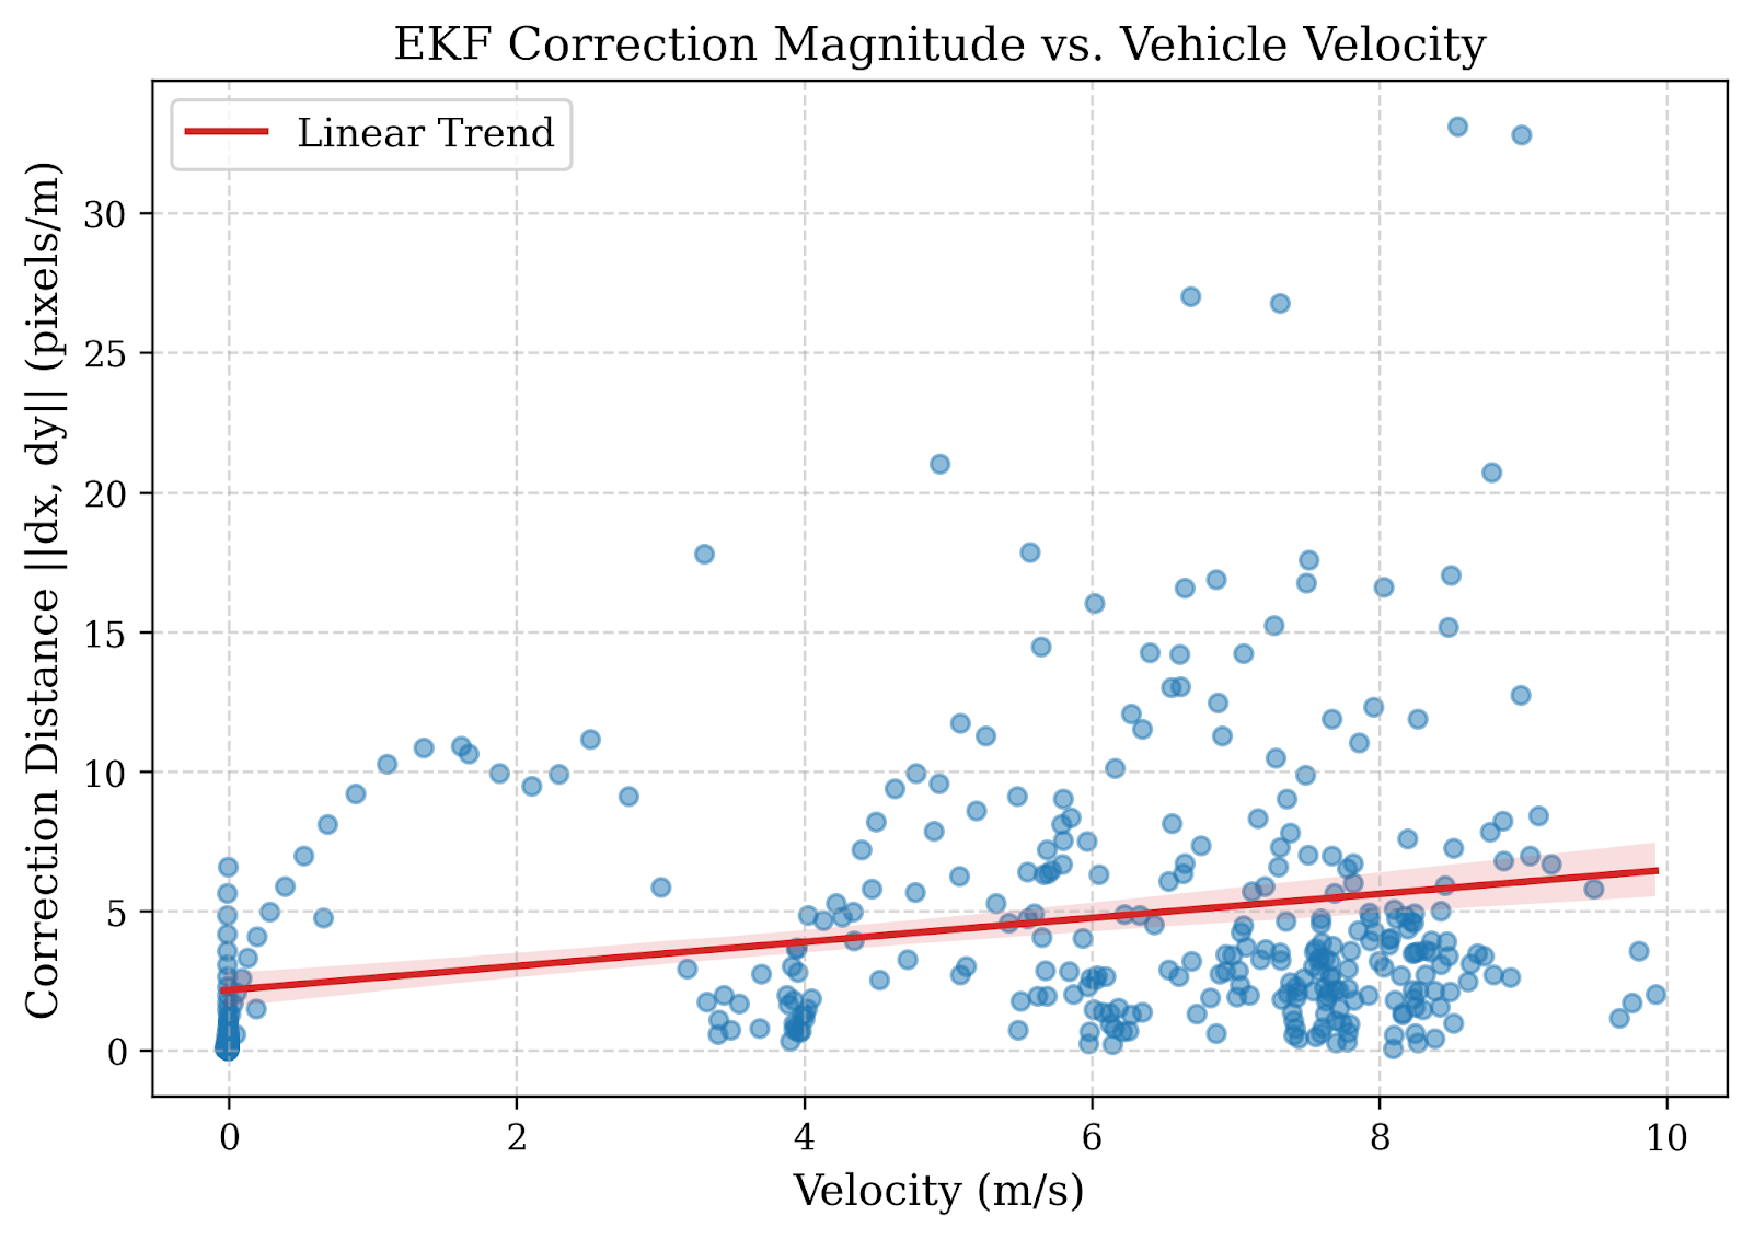
\includegraphics[width=0.8\textwidth]{figures/ekf_fig1_regression.pdf}
	\caption{\label{fig:ekf_regression}Linear regression analysis confirming a statistically significant positive correlation between vehicle velocity and EKF spatial correction magnitude $\Delta r = \|\mathbf{x}_{\text{smooth}} - \mathbf{x}_{\text{raw}}\|$.}
\end{figure}

As demonstrated in Figure~\ref{fig:ekf_regression}, the Euclidean correction distance $\Delta r = \sqrt{dx^2 + dy^2}$ exhibits a strong positive dependence on vehicle velocity. At low navigation speeds ($<2.5\text{ m/s}$), the median correction is only $0.43\text{ pixels/m}$, reflecting minor static background noise. However, as speed increases, the filter actively steps in to suppress dynamic vision errors.

% --- Figure 2: Boxplot Across Regimes ---
\begin{figure}[t]
	\centering
	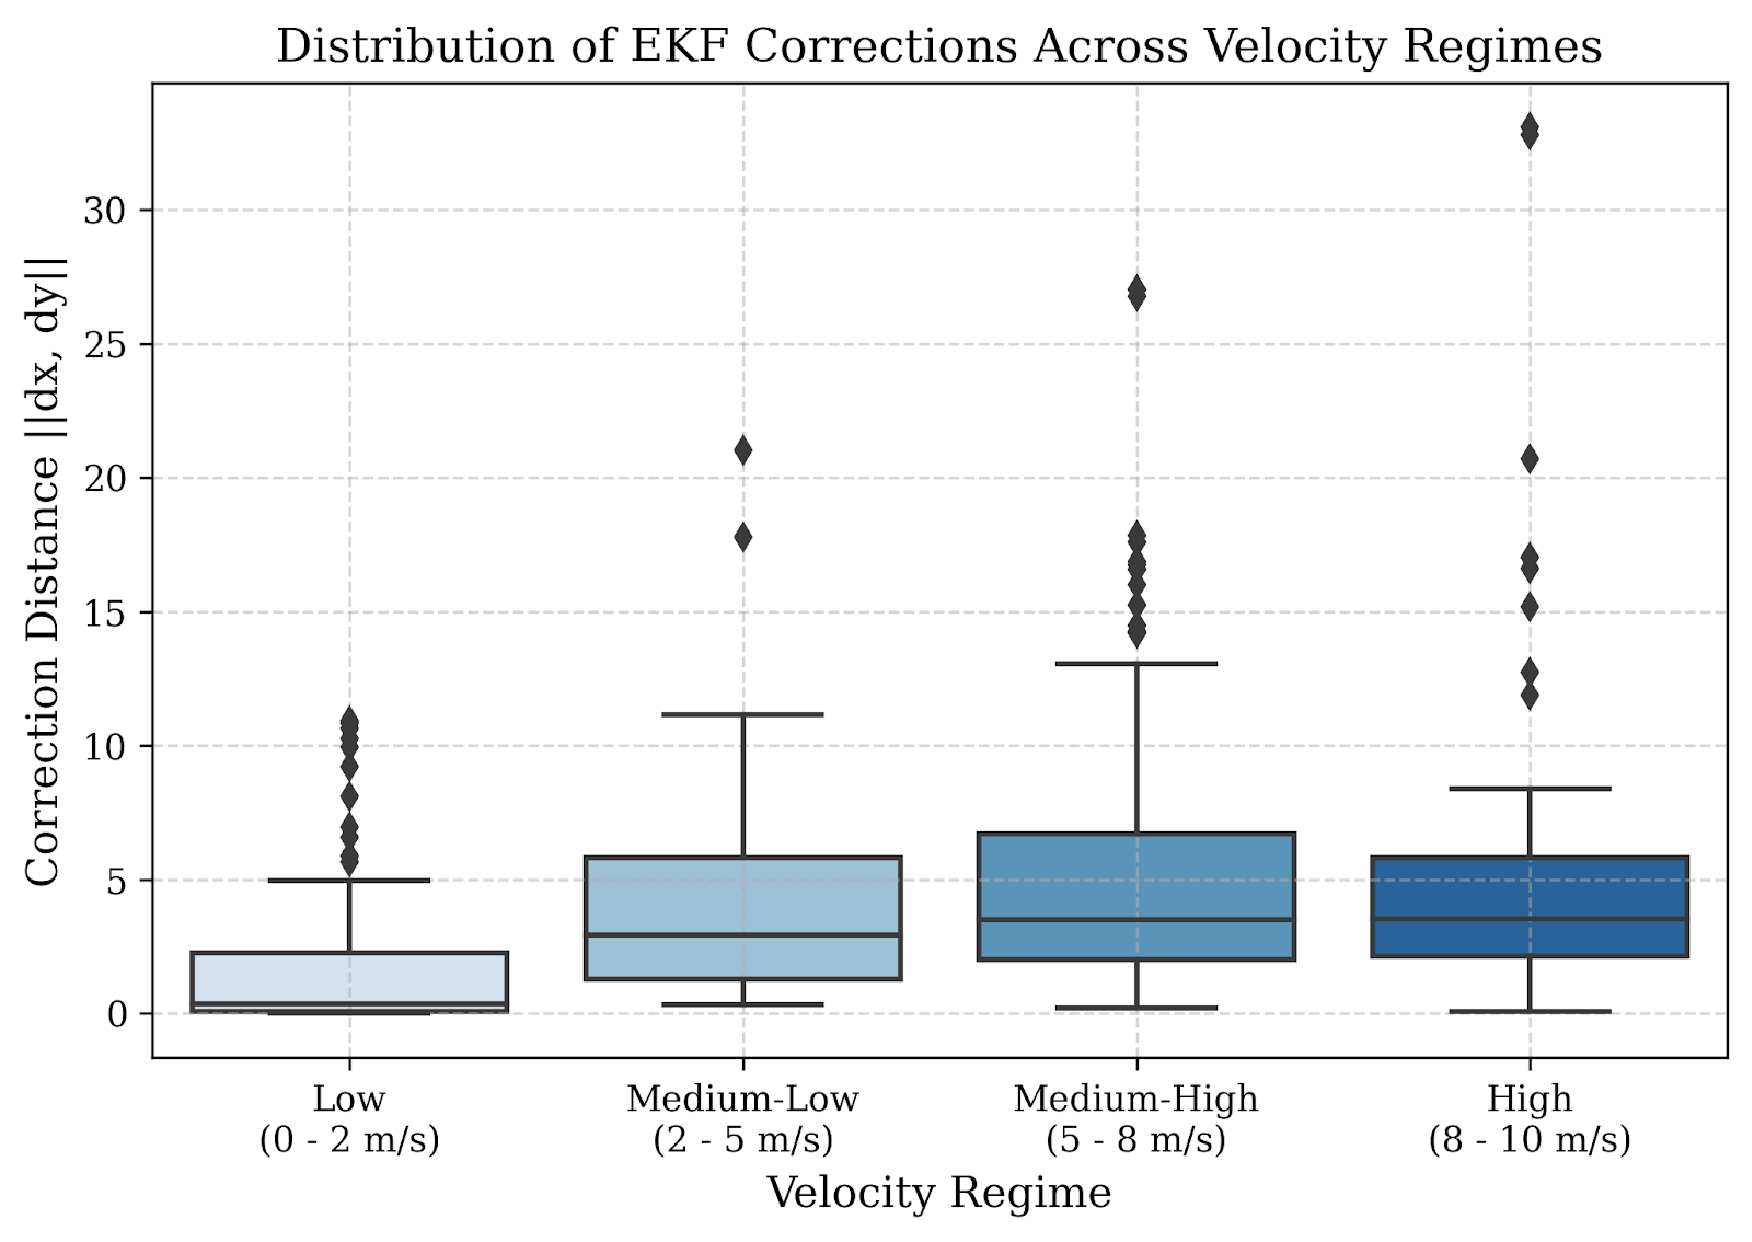
\includegraphics[width=0.8\textwidth]{figures/ekf_fig2_boxplot.pdf}
	\caption{\label{fig:ekf_boxplot}Distribution of EKF spatial corrections across four distinct velocity regimes, illustrating the upward shift in median and interquartile range at higher speeds.}
\end{figure}

This behavior is categorized across discrete speed brackets in Figure~\ref{fig:ekf_boxplot}. During high-velocity maneuvers ($>5.0\text{ m/s}$), the mean correction magnitude increases by over $180\%$ compared to idle regimes, with transient peak corrections reaching $33.10\text{ pixels/m}$.

% --- Figure 3: Temporal Alignment ---
\begin{figure}[t]
	\centering
	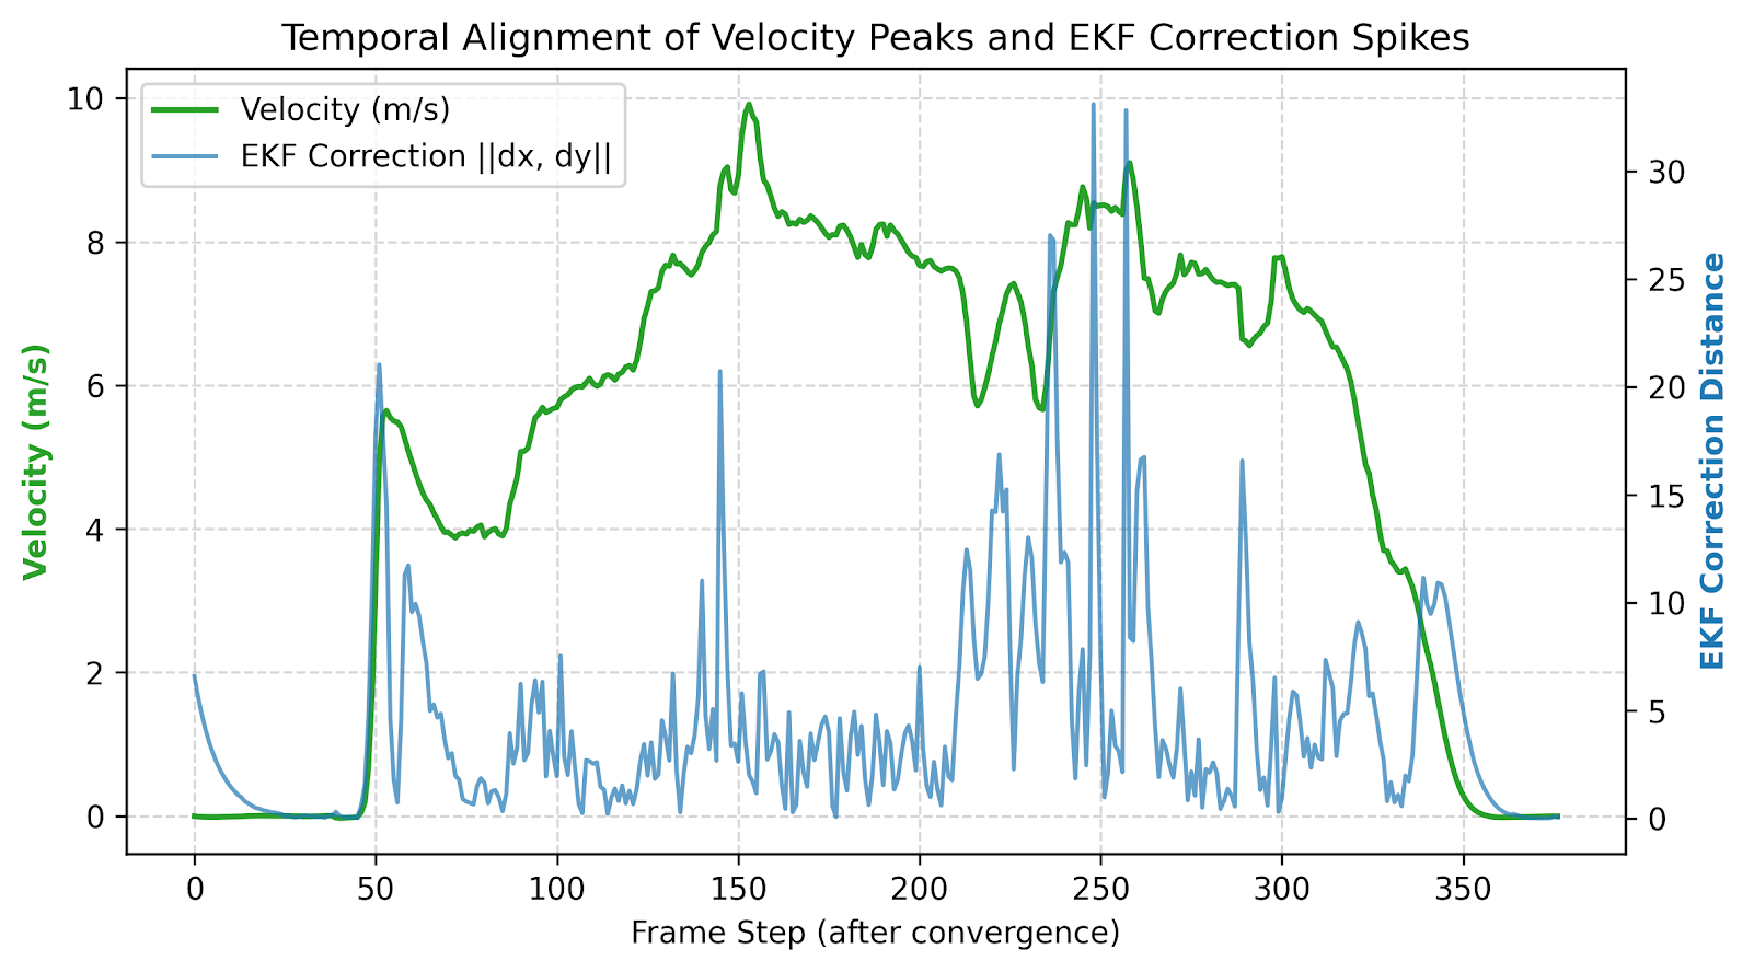
\includegraphics[width=0.85\textwidth]{figures/ekf_fig3_timeseries.pdf}
	\caption{\label{fig:ekf_timeseries}Temporal synchronization of vehicle velocity peaks (green) with EKF spatial correction intervention spikes (blue) over 377 post-convergence frames.}
\end{figure}

Rather than indicating filter instability, the temporal alignment displayed in Figure~\ref{fig:ekf_timeseries} provides quantitative proof of active kinematic damping. The continuous-time Constant Turn Rate and Velocity (\textsc{Ctrv}) dynamic model acts as a mathematical flywheel: while raw sensor observations experience severe spatial jitter during rapid acceleration, the filter dynamically intervenes precisely when velocity peaks occur.

% --- Figure 4: Spatial Trajectory Smoothing ---
\begin{figure}[t]
	\centering
	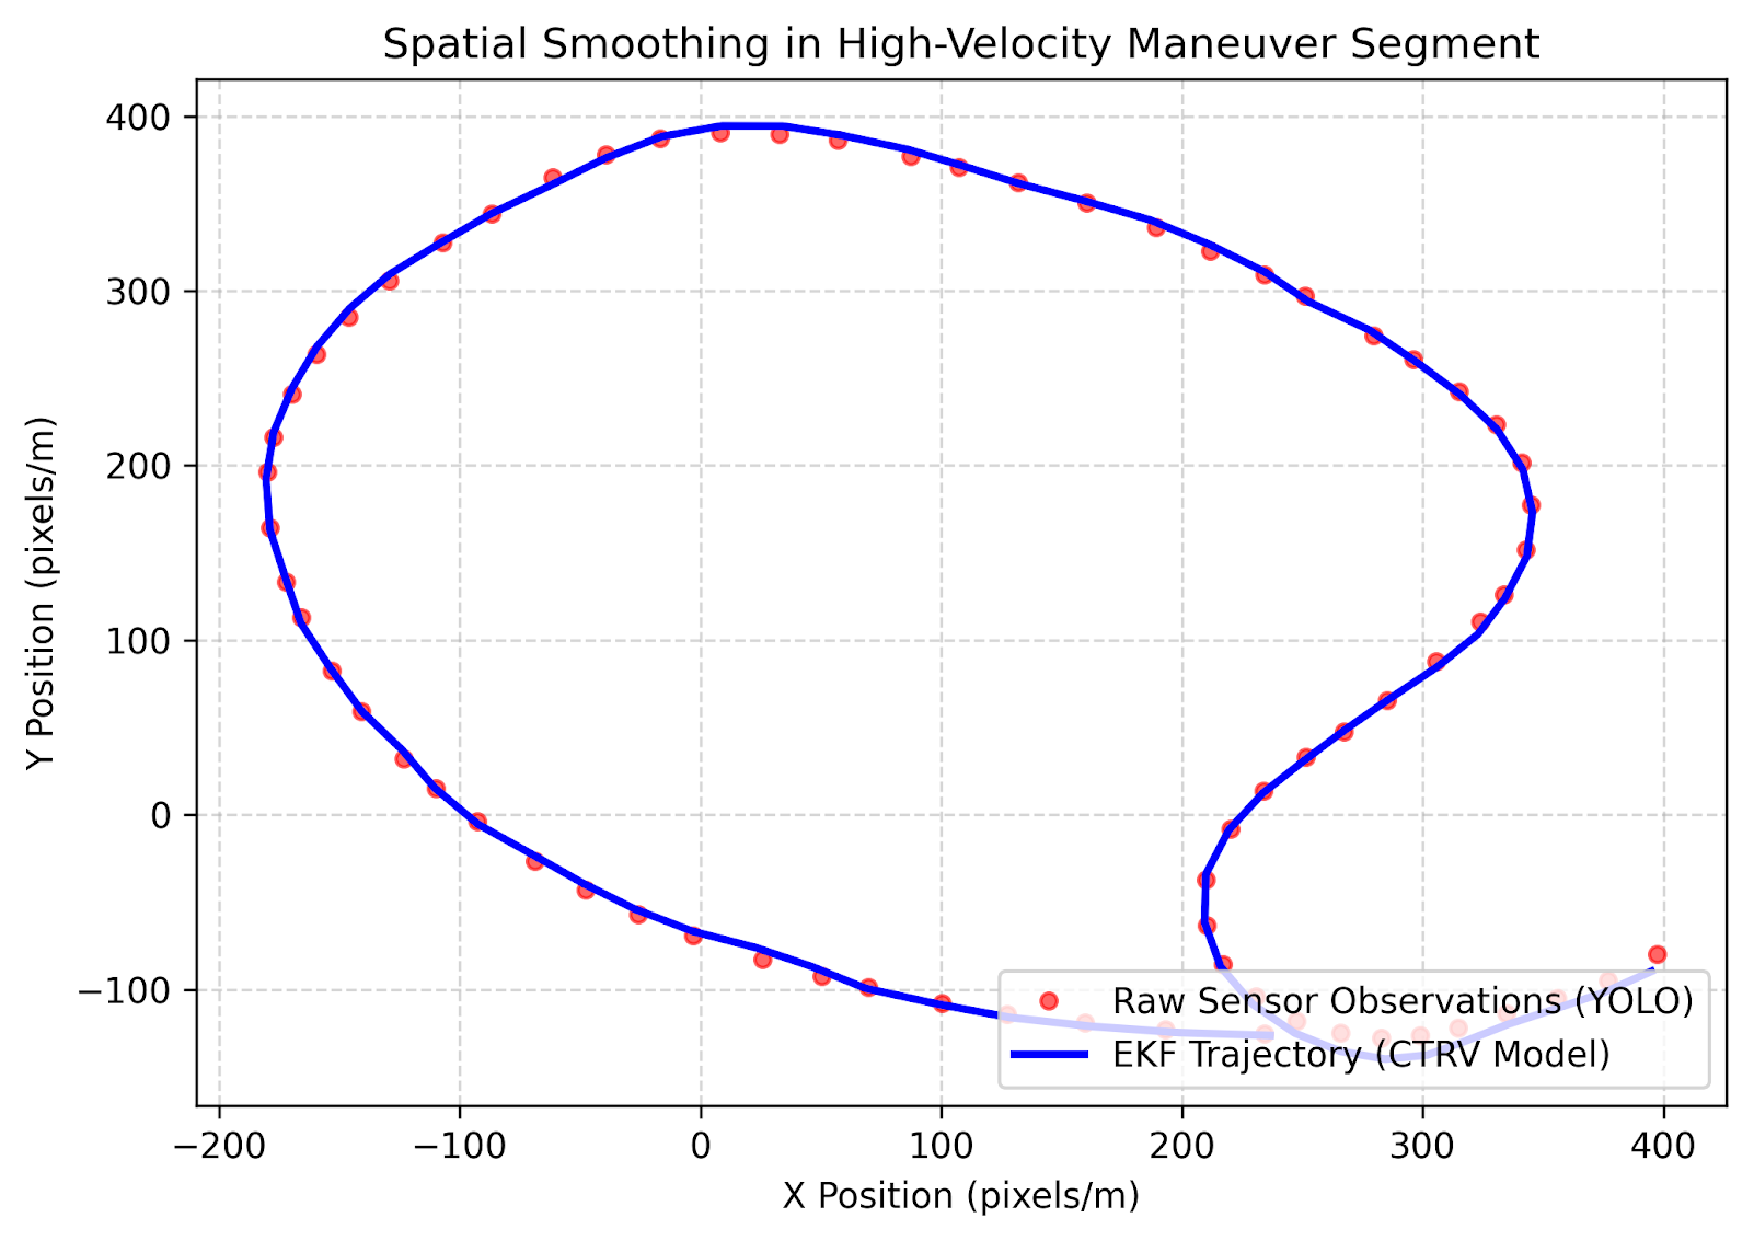
\includegraphics[width=0.8\textwidth]{figures/ekf_fig4_trajectory.pdf}
	\caption{\label{fig:ekf_trajectory}Spatial XY trajectory comparison during a high-speed maneuver segment (frames 150--220), highlighting the filter's ability to reject erratic raw sensor noise while maintaining physical momentum.}
\end{figure}

Finally, Figure~\ref{fig:ekf_trajectory} illustrates the spatial impact of this damping during a high-speed turning maneuver. The EKF propagates physical momentum forward, successfully isolating the true vehicular trajectory from high-frequency vision noise and bounding-box wobble.
